\ifdefined\XeTeXrevision\else\pdfoutput=1\fi
\documentclass[11pt,a4paper]{article}
\usepackage[utf8]{inputenc}
\usepackage[T1]{fontenc}
\usepackage{lmodern}
\usepackage{amsmath,amssymb,amsthm}
\usepackage{graphicx}
\graphicspath{{./}{figures/}{../figures/}}
\usepackage{booktabs}
\usepackage[hidelinks]{hyperref}
\usepackage[margin=1in]{geometry}
\usepackage{natbib}
\usepackage[inline]{enumitem}
\usepackage{xspace}
\usepackage{multirow}

\newtheorem{definition}{Definition}

\title{Explaining Benchmark Difficulty:\\Linear Logistic Test Models for\\Feature-Based AI Evaluation}

\author{Jung Min Kang\thanks{Corresponding author. Email: gangjeongmin23@gmail.com}\\
Independent Researcher\\
Seoul, South Korea}

\date{May 2026}

\begin{document}
\maketitle

\begin{abstract}
Standard Item Response Theory (IRT) corrects the ranking failures caused
by simple benchmark averaging under sparse evaluation conditions
\citep{kang2026scaling}, but treats each item as opaque---it estimates
\emph{how hard} items are without explaining \emph{why}. Recent work
predicts item difficulty from features via two-step pipelines that first
fit IRT, then regress on features \citep{ge2026agent}, or via
amortized joint models \citep{truong2025reliable}. We systematically
compare these approaches against the Linear Logistic Test Model (LLTM;
\citealp{fischer1973}), a classical psychometric framework that decomposes
item difficulty into observable features within a single likelihood
function. Across six experiments---including stress tests with irrelevant
features, omitted true features, and nonlinear difficulty
interactions---we find that: (1)~LLTM and two-step ridge regression
achieve comparable ranking recovery, both generally improving over unregularized standard IRT under
high sparsity, while remaining comparable to simple averaging for
ranking recovery; (2)~for predicting difficulty of
\emph{unseen} items, LLTM generally outperforms two-step ridge at lower
training fractions ($\rho = 0.87$ vs.\ $0.82$ at 50\% training data); and (3)~both methods show limited ranking-recovery degradation under
irrelevant features and moderate simulated misspecification. Neither
feature-based method consistently dominates the other for ranking;
the primary advantage of feature-based decomposition is the ability to
\emph{explain} difficulty sources and \emph{predict} difficulty for
new items---capabilities that enable principled benchmark design without
exhaustive model evaluation.
\end{abstract}


\section{Introduction}
\label{sec:intro}

\citet{kang2026scaling} demonstrated that simple averaging of benchmark
scores produces unreliable model rankings when evaluation data is sparse
and items vary in difficulty, with simple-average rankings degrading
substantially under sparse, heterogeneous evaluation matrices. Standard two-parameter logistic (2PL) IRT maintained
$\rho \geq 0.993$ across all conditions. However, standard IRT treats
each benchmark item as an opaque entity with a fixed difficulty parameter,
creating three practical limitations:

\begin{enumerate}[nosep]
\item \textbf{No prediction for new items.} Adding items to a benchmark
requires fresh evaluation data before difficulty can be estimated---a
single agentic evaluation run can cost over \$22{,}000
\citep{zhang2025darwin}.
\item \textbf{No explanation.} IRT reports item~47 has difficulty
$b = 1.83$, but not \emph{why}.
\item \textbf{Parameter scaling.} Standard 2PL requires $2K$ item-side
parameters, limiting estimation quality under sparse data.
\end{enumerate}

Recent work addresses these limitations by incorporating item features
into difficulty estimation. \citet{truong2025reliable} proposed an
amortized model-based evaluation framework that jointly trains IRT
ability parameters and a difficulty predictor from question content.
\citet{ge2026agent} extended this to agentic coding benchmarks, comparing
joint log-likelihood maximization against a two-step pipeline (fit IRT,
then ridge regression on features) and finding that two-step ridge
slightly outperformed joint training on held-out AUC-ROC.

These approaches implicitly rediscover a framework the psychometrics
community developed over fifty years ago: the \textbf{Linear Logistic
Test Model} (LLTM; \citealp{fischer1973}). LLTM replaces per-item
difficulty parameters with a linear combination of observable item
features, jointly estimating model abilities and feature weights within a
single likelihood function. Despite its extensive use in educational
measurement \citep{embretson2000,baghaei2017}, LLTM has not been
systematically evaluated for AI benchmark analysis.

This paper makes four contributions:
\begin{enumerate}[nosep]
\item We introduce LLTM to the AI evaluation literature with explicit
connections to recent feature-based approaches.
\item We provide a systematic comparison of LLTM, two-step ridge
regression, standard IRT, and simple averaging under controlled
conditions.
\item We stress-test all methods against noisy features, missing features,
and nonlinear difficulty interactions.
\item We demonstrate that feature-based decomposition---whether joint or
two-step---enables difficulty prediction for unseen items, with direct
implications for benchmark design.
\end{enumerate}


\section{Background}
\label{sec:background}

\subsection{Standard IRT}

The 2PL model specifies:
\begin{equation}
P(X_{ij} = 1 \mid \theta_i, a_j, b_j) = \sigma\bigl(a_j(\theta_i - b_j)\bigr)
\end{equation}
where $\theta_i$ is model ability, $b_j$ is item difficulty, and $a_j$
is item discrimination. The model requires $N + 2K$ parameters.

\subsection{The Linear Logistic Test Model}

\citet{fischer1973} proposed decomposing difficulty as:
\begin{equation}
b_j = \sum_{f=1}^{F} w_f \cdot q_{jf} + c
\end{equation}
where $q_{jf}$ is feature~$f$ for item~$j$ and $w_f$ is the learned
weight. Substituting yields:
\begin{equation}
P(X_{ij} = 1 \mid \theta_i, \mathbf{w}) = \sigma\!\left(\theta_i - \sum_{f=1}^{F} w_f \cdot q_{jf}\right)
\label{eq:lltm}
\end{equation}
Item-side parameters reduce from $2K$ to $F$ (typically $F \ll K$).

LLTM belongs to the Rasch/1PL family with linear constraints on item
parameters \citep{fischer1973}. It is more constrained than standard 2PL;
under sparse data, this constraint acts as regularization. Under
well-specified features, the constraint is approximately correct and
estimation benefits. Under misspecified features, the constraint may hurt.
We test both scenarios.

\subsection{Two-Step Feature Regression}

\citet{ge2026agent} proposed: (1)~fit standard IRT to obtain
$\hat{b}_j$; (2)~fit ridge regression
$\hat{b}_j \approx \sum_f w_f q_{jf}$. This avoids joint optimization
but propagates estimation uncertainty from step~1.
\citet{ge2026agent} found this two-step approach slightly outperformed
their joint log-likelihood variant on held-out AUC-ROC for agentic coding
benchmarks.

\subsection{Amortized Model-Based Evaluation}

\citet{truong2025reliable} proposed jointly training IRT ability
parameters and a difficulty predictor, using the predicted difficulty to
enable efficient evaluation of new models. Their approach is conceptually
closest to LLTM but uses neural architectures for the difficulty
predictor.


\section{Experimental Design}
\label{sec:method}

\subsection{Data Generation}

We simulate benchmark data with $N = 25$ models, $K = 100$ items, and
$F = 5$ observable item features (Table~\ref{tab:features}). True item
difficulty is a weighted linear combination of features plus Gaussian
noise ($\sigma = 0.3$). Item discrimination is sampled uniformly from
$[0.5, 2.0]$. Responses are sampled from a 2PL model. Each condition
uses 5~independent random seeds.

\begin{table}[h]
\centering
\small
\caption{Simulated item features and true generative weights.}
\label{tab:features}
\begin{tabular}{llr}
\toprule
Feature & Description & True $w$ \\
\midrule
Reasoning depth & Inferential steps required & 1.5 \\
Domain specificity & Specialized knowledge required & 0.8 \\
Prompt complexity & Structural complexity of prompt & 0.6 \\
Answer ambiguity & Ambiguity in correct response & 1.2 \\
Context length & Required context processing & 0.3 \\
\bottomrule
\end{tabular}
\end{table}

\subsection{Methods Compared}

\begin{enumerate}[nosep]
\item \textbf{Simple averaging.} Mean accuracy per model.
\item \textbf{Standard 2PL IRT.} Alternating MLE with unconstrained
item parameters and no regularization. This baseline is intentionally
unregularized; comparison against regularized, Bayesian, and
Rasch-family IRT estimators is left to future work.
\item \textbf{LLTM (joint).} Joint estimation of abilities and feature
weights via alternating MLE with L2 regularization ($\lambda = 0.01$).
\item \textbf{Two-step ridge.} Standard IRT followed by ridge regression
on features, following \citet{ge2026agent}.
\end{enumerate}

\subsection{Experiments}

\begin{enumerate}[nosep]
\item \textbf{Sparsity sweep.} Missing data rate from 0\% to 90\%.
\item \textbf{Noisy features.} Add 0--20 irrelevant random features.
\item \textbf{Missing true feature.} Remove the strongest feature
(reasoning depth, $w = 1.5$).
\item \textbf{Nonlinear interactions.} Add interaction term
$0.8 \cdot \text{reasoning} \times \text{ambiguity}$.
\item \textbf{Unseen item prediction.} Train on 30--90\% of items,
predict difficulty for held-out items.
\item \textbf{Feature weight recovery.} Compare learned weights to
ground truth.
\end{enumerate}


\section{Results}
\label{sec:results}

\subsection{Ranking Recovery Under Sparsity}

Table~\ref{tab:sparsity} reports ranking recovery across sparsity
conditions. At full data, LLTM and two-step perform identically
($\rho = 0.992$). Under sparsity, both feature-based methods
generally improve over unregularized standard IRT, with the clearest
gap at 90\% missing data. At 90\% missing, two-step ridge ($\rho = 0.889$)
matches simple averaging, while LLTM ($\rho = 0.883$) is slightly
lower.

\textbf{Key finding:} The primary benefit of feature-based methods over
standard IRT is not that one dominates the other, but that \emph{both}
improve over unconstrained IRT under sparsity
by leveraging item features for implicit regularization.

\begin{table}[t]
\centering
\small
\caption{Ranking recovery (Spearman~$\rho$, mean over 5 seeds).
Bold: best per row. LLTM and two-step achieve comparable performance,
generally improving over unregularized standard IRT at higher sparsity.}
\label{tab:sparsity}
\begin{tabular}{lcccc}
\toprule
Missing & Averaging & IRT (2PL) & LLTM & Two-Step \\
\midrule
0\%  & \textbf{0.992} & 0.989 & \textbf{0.992} & \textbf{0.992} \\
30\% & 0.988 & 0.980 & \textbf{0.988} & \textbf{0.988} \\
50\% & 0.981 & 0.969 & 0.984 & \textbf{0.984} \\
70\% & 0.956 & 0.946 & \textbf{0.961} & 0.958 \\
90\% & \textbf{0.889} & 0.841 & 0.883 & \textbf{0.889} \\
\bottomrule
\end{tabular}
\end{table}

\begin{figure}[t]
\centering
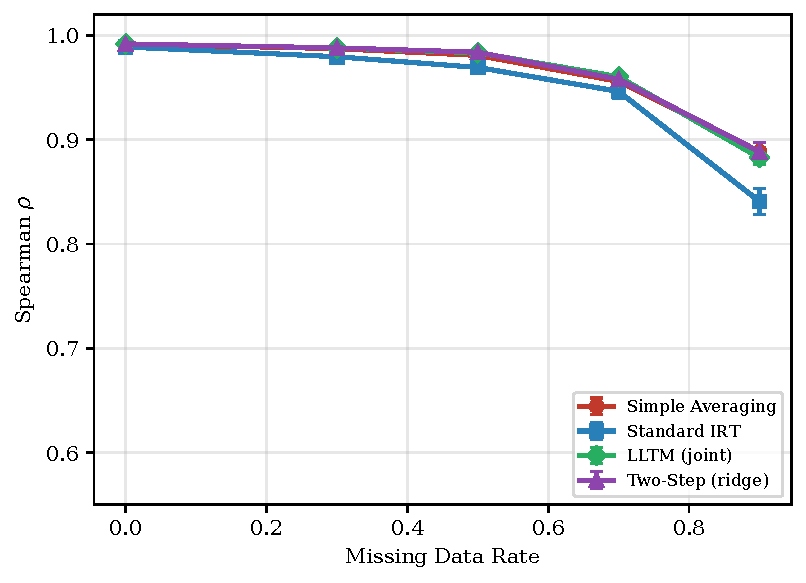
\includegraphics[width=0.85\linewidth]{fig1_sparsity.pdf}
\caption{Ranking recovery under increasing sparsity. LLTM and two-step
ridge both improve over unregularized 2PL IRT under sparsity, while
remaining comparable to simple averaging. Neither feature-based method
uniformly dominates the other. Error bars show $\pm 1$ SE.}
\label{fig:sparsity}
\end{figure}

\subsection{Stress Tests}

Figure~\ref{fig:stress} reports results for four stress tests.

\paragraph{Noisy features (Fig.~\ref{fig:stress}a).}
Adding up to 20 irrelevant features causes minimal degradation for both
methods. LLTM maintains $\rho \geq 0.991$ with 20 noise features,
slightly outperforming two-step ($\rho = 0.986$).
This pattern is consistent with regularization suppressing
irrelevant feature weights.

\paragraph{Missing true feature (Fig.~\ref{fig:stress}b).}
When the strongest feature (reasoning depth, $w = 1.5$) is hidden from
the model but still affects true difficulty, ranking recovery is
unaffected at full data and \emph{slightly improves} under sparsity
(LLTM: $0.974$ vs.\ $0.967$ with all features at 70\% missing).
This counterintuitive result occurs because removing a feature reduces
model complexity, providing stronger regularization when data is scarce.
Note that this robustness applies to \emph{ranking recovery}; the impact
on difficulty prediction accuracy under omitted features remains an open
question for future work.

\paragraph{Nonlinear interactions (Fig.~\ref{fig:stress}c).}
Adding a reasoning~$\times$~ambiguity interaction causes minimal
degradation at full data but a small drop under sparsity for LLTM
($0.961 \to 0.953$ at 70\% missing). Two-step ridge is slightly more
robust to nonlinearity under sparsity ($0.960 \to 0.959$).

\paragraph{Unseen item prediction (Fig.~\ref{fig:stress}d).}
LLTM outperforms two-step ridge for difficulty prediction at 70\%,
50\%, and 30\% training fractions, with the clearest advantage under
lower training coverage. At 30\% training, LLTM shows the largest
observed gap:
$\rho = 0.856$ vs.\ $0.797$. At 90\% training, two-step is slightly
higher ($0.770$ vs.\ $0.760$), likely reflecting noise from the small
held-out set. Standard IRT cannot perform this task at all.

\begin{figure}[t]
\centering
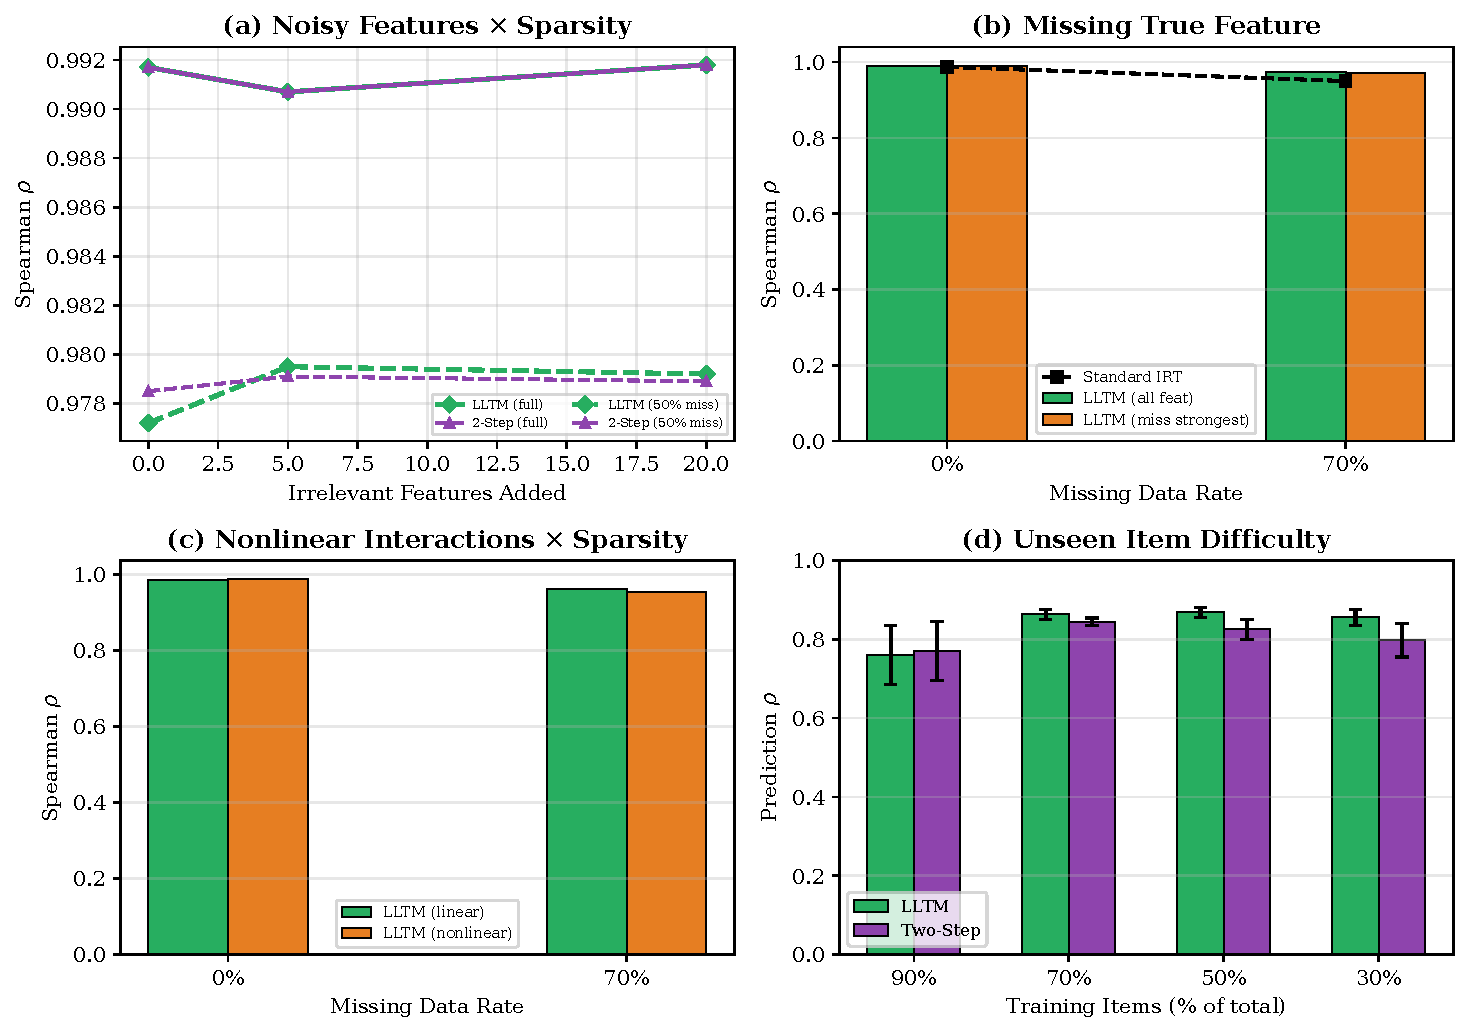
\includegraphics[width=\linewidth]{fig2_stress.pdf}
\caption{Stress tests. (a)~Both methods show limited degradation under
irrelevant features, including under 50\% sparsity. (b)~Hiding the strongest feature causes minimal degradation in ranking
recovery, though its effect on difficulty prediction remains untested.
(c)~Moderate nonlinearity does not substantially affect either method.
(d)~LLTM generally outperforms two-step ridge for difficulty prediction
at lower training fractions; at 90\% training, two-step is slightly
higher.}
\label{fig:stress}
\end{figure}

\subsection{Feature Weight Recovery}

Both LLTM and two-step ridge recover the true feature importance ranking
with $\rho = 0.90$ (Figure~\ref{fig:weights}), correctly identifying
reasoning depth and answer ambiguity as the strongest difficulty
predictors. The learned weights enable benchmark designers to understand
which item characteristics drive difficulty and to control difficulty
distributions when constructing new benchmarks.

\begin{figure}[t]
\centering
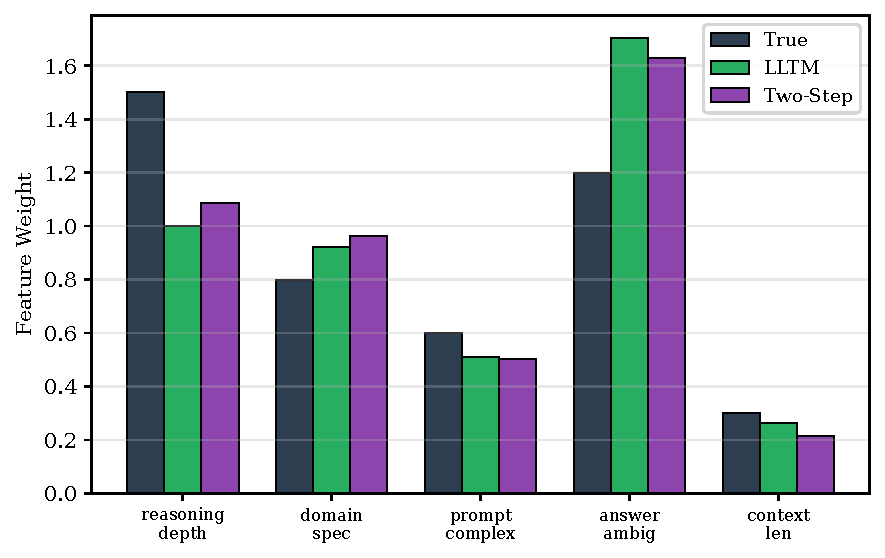
\includegraphics[width=0.85\linewidth]{fig3_weights.pdf}
\caption{Feature weight recovery. Both LLTM and two-step correctly
identify the relative importance of difficulty predictors.}
\label{fig:weights}
\end{figure}

\subsection{Parameter Efficiency}

LLTM requires $N + F$ parameters (25 + 5 = 30) compared to $N + 2K$
for standard IRT (25 + 200 = 225)---an 87\% reduction in total
parameters. For benchmarks with $K = 1{,}000$ items, item-side
parameters drop by 99.75\% (from 2{,}000 to~5); total parameters
drop by 98.5\% (from 2{,}025 to~30).


\section{Discussion}
\label{sec:discussion}

\paragraph{From diagnosis to design.}
\citet{kang2026scaling} diagnosed when evaluation fails. Feature-based
difficulty decomposition provides a constructive tool: by revealing
which features drive difficulty, it enables benchmark designers to
predict difficulty for candidate items before evaluation, control
difficulty distributions, and identify under-represented item types.

\paragraph{Joint vs.\ two-step estimation.}
Classical psychometric theory favors joint estimation because it avoids
propagating errors across stages \citep{deboeck2004}. However,
\citet{ge2026agent} found that two-step ridge slightly outperformed
joint log-likelihood on their agentic coding data. Our results add
nuance: for \emph{ranking recovery}, LLTM and two-step perform
comparably across all conditions tested. For \emph{difficulty
prediction on unseen items}, LLTM shows its largest observed advantage
at lower training fractions in this controlled simulation ($\rho = 0.856$
vs.\ $0.797$ at 30\% training). This suggests the choice depends on the
application: two-step when simplicity and modularity are prioritized;
joint estimation when difficulty prediction and benchmark design are
central.

\paragraph{Limitations.}
This study uses simulated data where difficulty is generated from a
linear feature model, which is structurally favorable to LLTM. Our
stress tests show limited degradation in ranking recovery under
irrelevant features, omitted
true features, and moderate nonlinear interactions, but stronger
misspecification (e.g., fully nonlinear difficulty, high-dimensional
feature noise under extreme sparsity) remains untested. Validation
on real benchmark data---such as the agentic coding tasks from
\citet{ge2026agent} or HELM---is needed before strong generalization
claims. LLTM's 1PL constraint (no per-item discrimination) may limit
fit on benchmarks where items differ substantially in discriminative
power.

\paragraph{Relationship to prior work.}
Both \citet{truong2025reliable} and \citet{ge2026agent} independently
developed feature-based difficulty prediction for AI evaluation. Our
contribution is connecting these developments to Fischer's classical
LLTM framework, providing systematic stress tests, and emphasizing the
benchmark \emph{design} application that existing work does not explore.


\section{Conclusion}
\label{sec:conclusion}

Feature-based difficulty decomposition---whether via LLTM's joint
estimation or two-step ridge regression---addresses a fundamental
limitation of standard IRT for AI evaluation: it explains why items
are hard, predicts difficulty for unseen items, and does so with
dramatically fewer parameters. The primary advantage is not ranking
accuracy (where simple averaging remains competitive) but the ability
to understand and control benchmark difficulty. As AI evaluation scales
to thousands of items across multiple domains, these capabilities become
essential for principled benchmark design.

\paragraph{Reproducibility.}
All experiments are implemented in a single NumPy/SciPy script
requiring no deep learning frameworks or GPU resources.
Complete code, including data generation, estimation, and
figure plotting, is included in the supplementary materials.

\bibliographystyle{plainnat}
\bibliography{references}

\appendix
\section{Simulation Code}
\label{app:code}
The complete experiment script (\texttt{experiment.py}) is included in
the submission archive and generates all results and figures reported
in this paper. Key parameters: $N = 25$ models, $K = 100$ items,
$F = 5$ features, 5 random seeds per condition.

\end{document}
